\section{Introduction}
\label{sec:introduction}

GPUs are among the most expensive and contended resources in modern computing infrastructure, which makes them an attractive target for cryptomining abuse. Clusters and cloud GPU pools run workloads that are long-lived and compute intensive, so an unauthorized miner can quietly consume accelerator resources while looking much like an ordinary compute-bound job. The financial incentive is direct: the miner profits while the operator pays for hardware that should be serving legitimate research work.

Existing GPU cryptojacking defenses infer mining from \emph{indirect} evidence rather than from the computation that is actually submitted to the GPU. They watch network traffic, host behavior, GPU telemetry~\cite{pott2023gpucryptojacking,tanana2024gpucryptojacking}, or physical side channels~\cite{xiao2023magtracer,cao2025maginspector}. Such signals can show that a GPU is busy or that kernels launch repeatedly, but they do not answer the security question directly: whether the submitted GPU code implements a mining search loop or a legitimate high-throughput kernel.

We present \emph{GPU-Sentry}, a system for instruction-level detection of cryptomining-like GPU computation. GPU-Sentry transparently captures GPU code objects and kernel-launch events at the CUDA Driver API boundary, reconstructs and normalizes the submitted GPU assembly (SASS, the native instruction set that NVIDIA GPUs execute), and builds stream-level instruction windows over the kernel launch sequence. A ModernBERT~\cite{warner2024modernbert} sequence classifier then labels each normalized window as mining-like or benign.

The central insight is that mining stays visible in the instruction stream even when host-level evidence is weak. A user can rename processes, obfuscate the host binary, throttle the launch loop, or co-run mining beside benign jobs; these evasions alter names, timing, and surrounding activity, but the GPU must still receive the executable kernels that perform the mining computation. GPU-Sentry therefore treats the submitted GPU program as the primary evidence; device telemetry serves only as a comparison baseline in our evaluation. \Cref{tab:feature_comparison} summarizes how this evidence differs from that exposed by prior detection approaches. To the best of our knowledge, GPU-Sentry is the first system to detect GPU cryptomining from the GPU instructions (normalized SASS) actually submitted to the device, rather than from indirect signals such as GPU telemetry, performance counters, or physical side channels.

\begin{table*}[t]
    \centering
    \caption{Detection approaches expose different evidence. GPU-Sentry inspects the submitted GPU computation and attributes it to CUDA execution context. ($\checkmark$ yes, $\times$ no, $\sim$ partial)}
    \label{tab:feature_comparison}
    \footnotesize
    \begin{tabular}{lccccc}
        \toprule
        Capability & Network / flow & Behavioral telemetry & Physical side channel & Static binary analysis & \textbf{GPU-Sentry} \\
        \midrule
        Sees the submitted GPU computation & $\times$ & $\times$ & $\times$ & $\sim$ & \textbf{$\checkmark$} \\
        Robust to process or kernel renaming & $\checkmark$ & $\checkmark$ & $\checkmark$ & $\times$ & \textbf{$\checkmark$} \\
        Robust to encrypted network traffic & $\times$ & $\checkmark$ & $\checkmark$ & $\checkmark$ & \textbf{$\checkmark$} \\
        Robust to host binary obfuscation & $\checkmark$ & $\checkmark$ & $\checkmark$ & $\times$ & \textbf{$\checkmark$} \\
        Robust to throttled mining & $\times$ & $\times$ & $\times$ & $\checkmark$ & \textbf{$\checkmark$} \\
        Robust to mixed benign \& mining on the same GPU & $\times$ & $\times$ & $\times$ & $\checkmark$ & \textbf{$\checkmark$} \\
        Pinpoints the mining process & $\sim$ & $\times$ & $\times$ & $\checkmark$ & \textbf{$\checkmark$} \\
        No special hardware or sensors required & $\checkmark$ & $\checkmark$ & $\times$ & $\checkmark$ & \textbf{$\checkmark$} \\
        \bottomrule
    \end{tabular}
\end{table*}

Building a usable instruction-level detector raises several practical challenges. GPU code arrives in many forms: PTX, fatbins, or CUBINs, from files or memory. Users submit it through diverse libraries, frameworks, and containers, so it must be captured however it is submitted, without user intervention. The same computation compiles to different SASS across GPU architectures, compiler versions, and optimization levels. A miner may launch one kernel repeatedly or split its work across helper kernels, so single launches are not the right unit of analysis. And public GPU-miner datasets are scarce. We develop these challenges and the mechanisms that address them in \cref{sec:motivation}.

GPU-Sentry addresses these challenges with the following contributions:
\begin{itemize}
    \item a transparent CUDA Driver API capture layer that records GPU code objects and launch events for system-wide native and containerized workloads;
    \item a normalized SASS representation with control-flow-driven main-loop extraction and architecture-aware opcode-family mapping;
    \item a per-stream window scheduler that assembles launches into model-sized windows and deduplicates them by kernel-composition signature;
    \item a ModernBERT detector that classifies each normalized instruction window as mining-like or benign; and
    \item a synthetic-to-real training and evaluation workflow that trains the detector entirely on synthetic normalized SASS and shows that this training transfers to real-world GPU captures.
\end{itemize}

\section{Background and Threat Model}
\label{sec:background}

\subsection{CUDA Code and Execution}

CUDA applications reach the GPU through a layered software stack, shown in \cref{fig:cuda_stack}. An application may call the CUDA Runtime API directly, use a CUDA library such as cuBLAS or cuDNN, or run on top of a framework such as PyTorch or TensorFlow. These layers ultimately use the CUDA Driver API~\cite{nvidiaCudaDriverAPI} to load code modules, resolve kernel handles, and launch kernels on CUDA streams. A stream is an ordered execution queue, so launches issued on the same stream preserve program order even when other streams run concurrently. The CUDA Driver API is therefore the narrow waist that every CUDA application must traverse, regardless of the higher-level interface the application uses.

\begin{figure}[t]
    \centering
    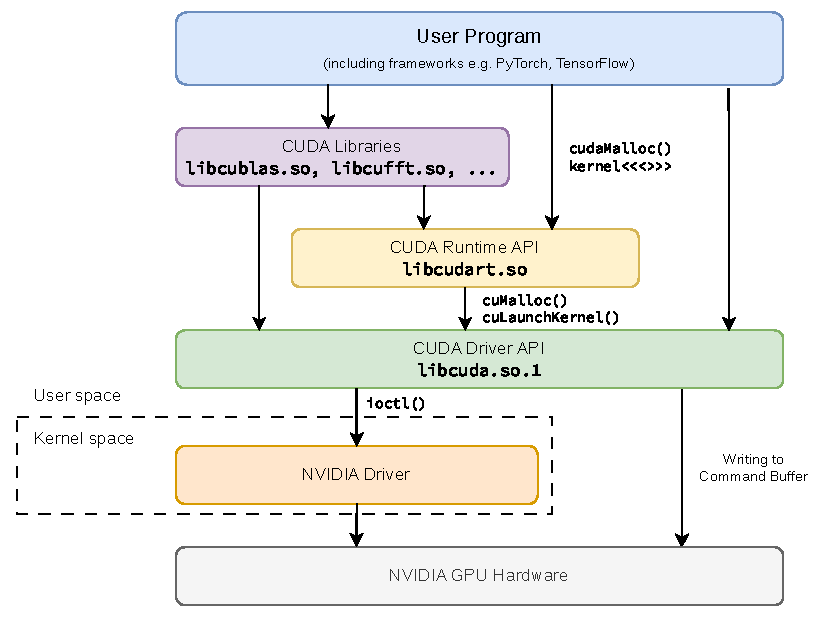
\includegraphics[width=0.86\columnwidth]{Figures/CUDAAPIs.pdf}
    \caption{The CUDA software stack. Applications, libraries, the Runtime API, and frameworks all reach the GPU through the CUDA Driver API, which loads code objects and launches kernels.}
    \label{fig:cuda_stack}
\end{figure}

GPU code appears in several representations before execution. PTX is a virtual instruction set that is just-in-time compiled for a target GPU. SASS is the native instruction set of a specific GPU architecture and the final representation that NVIDIA hardware executes. A CUBIN is a binary for a single GPU architecture, and its machine code is SASS; a fatbin bundles one or more CUBINs, often alongside PTX, so the loader can select the variant matching the GPU in use.

\subsection{Threat Model}

GPU-Sentry assumes a monitored host whose administrator controls the CUDA driver deployment and the GPU-Sentry collector. An unprivileged user may run arbitrary CUDA applications on the host or inside a container. The user's miner uses CUDA and is initiated through the system's CUDA software stack.

The user actively hides the miner's intent but cannot modify the parts of the system we trust. Specifically, the user may rename processes and kernels, strip symbols, pack or obfuscate the host binary, compile a custom miner, change optimization levels, throttle the kernel-launch loop, and co-run mining with benign GPU work. We assume the user cannot control the host administrator, the kernel-mode driver, or the GPU-Sentry collector. CPU-only mining is out of scope because it never reaches the GPU. We also assume the user does not replace or bypass the monitored userspace CUDA driver that GPU-Sentry interposes on; because that driver is a userspace library, a same-privilege user could in principle do so, a deployment limitation we discuss in \cref{sec:limitations}.

\section{Motivation and Design Challenges}
\label{sec:motivation}

\subsection{Telemetry Is Not Enough}

Telemetry-based detection is easy to deploy but cannot identify the submitted computation. Device counters---GPU utilization, memory use, power draw, and temperature---can flag a miner that runs alone on an otherwise idle or lightly loaded GPU, but two effects break this in shared HPC and AI clusters. First, many benign GPU applications are themselves resource-intensive, so high utilization is not distinctive. Second, a miner can move its device-level footprint into ordinary-looking ranges by throttling its launch loop or running beside benign work. In these cases telemetry describes the \emph{effect} of execution, not the \emph{code} that produced it, which makes it prone to both false positives and false negatives.

Our reimplementation of GPU-counter detection following Pott et al.~\cite{pott2023gpucryptojacking}---a Random Forest over whole-device measurements---shows this. It is highly accurate on ordinary isolated runs, but its accuracy drops sharply once the miner throttles its kernel-launch loop or runs beside a benign job (\cref{sec:evaluation}). Throttling spreads the mining activity thinly over time, and a co-running benign job hides it behind its own heavy device usage. GPU-Sentry instead reads normalized SASS windows, so throttling changes only \emph{when} a window fills, not the kernel body that is eventually analyzed.

\subsection{Design Challenges}

Building an instruction-level detector raises six practical challenges, listed below.

\begin{itemize}
    \item \textbf{Code-object diversity.} GPU code arrives as PTX, fatbins, or CUBINs, from files or memory. GPU-Sentry hooks all Driver-API module and library loads and captures the SASS actually submitted to the device (\cref{sec:capture}).
    \item \textbf{Transparent capture across workloads.} Workloads span native programs, libraries, frameworks, and containers. GPU-Sentry interposes a replacement \texttt{libcuda.so.1} at the Driver-API boundary, propagated into containers through the NVIDIA Container Toolkit (\cref{sec:capture}).
    \item \textbf{Repeated and split kernels.} A miner may launch one kernel repeatedly or split work across helper kernels. GPU-Sentry analyzes stream-level instruction windows, each filled to the token budget and deduplicated by kernel-composition signature (\cref{sec:windows}).
    \item \textbf{SASS variation.} SASS is architecture-specific: newer GPU generations add new instructions and rename or retire others. GPU-Sentry normalizes operands and maps architecture-specific opcodes to common semantic families (\cref{sec:normalization}).
    \item \textbf{Compiler and optimization variation.} Code differs across compiler versions and optimization levels. GPU-Sentry combines the normalized representation with multi-optimization (O2/O3) training and leakage-aware splits (\cref{sec:dataset}).
    \item \textbf{Scarce cryptominer training data.} There is no public GPU-miner dataset and few collectable real miners. GPU-Sentry trains on synthetic workloads and reserves all real captures for evaluation (\cref{sec:dataset}).
\end{itemize}

\section{System Design}
\label{sec:design}

\subsection{Overview}
\label{sec:design_overview}

GPU-Sentry turns opaque CUDA activity into auditable instruction-level evidence. \Cref{fig:architecture} shows the architecture. A client-side CUDA interception library captures code-load and launch events and forwards them asynchronously to the collector, keeping the application-facing CUDA path lightweight. The server-side analysis pipeline then reconstructs code objects, normalizes their SASS, builds stream-local launch windows, renders each window as an instruction sequence, and sends the sequence to the ModernBERT detector. The detector returns a mining score and a verdict that can be logged, reported, or used to terminate the offending process under an administrator-defined policy. Captured artifacts are archived to disk for later audit.

\begin{figure*}[t]
    \centering
    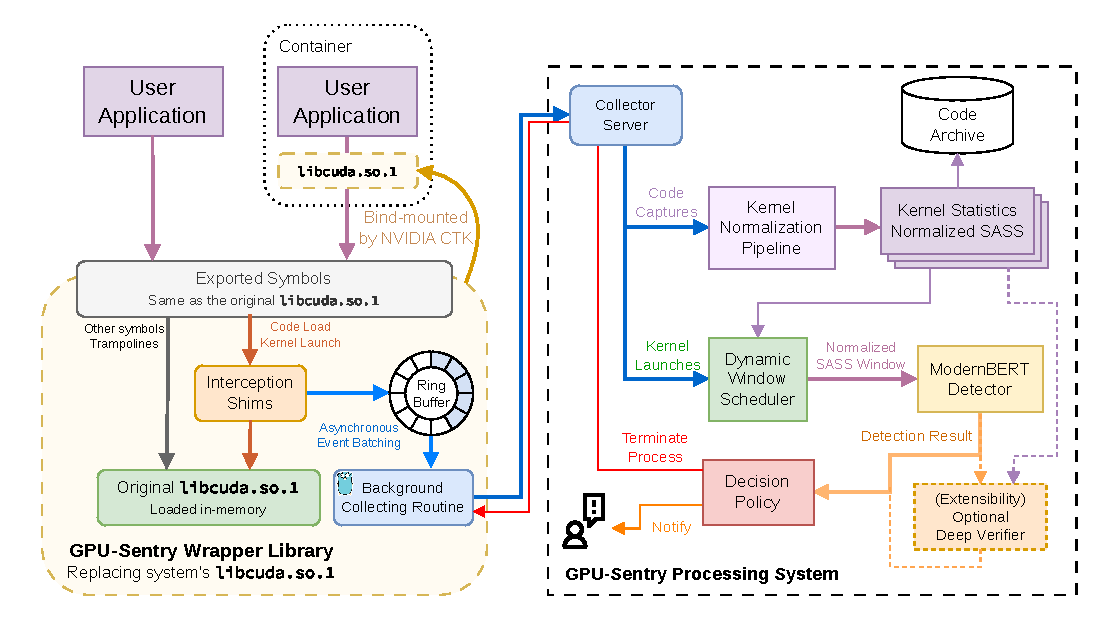
\includegraphics[width=0.92\textwidth]{Figures/Architecture}
    \caption{GPU-Sentry architecture. The interception library records CUDA's module code load and launch activity; the server-side analysis pipeline reconstructs normalized SASS, builds stream-level windows with the window scheduler, and invokes the ModernBERT detector, which produces a verdict. An optional verification layer (dashed) can be added but is not used in our evaluation.}
    \label{fig:architecture}
\end{figure*}

The design separates capture from analysis because CUDA calls are latency-sensitive. The interception path only creates compact events and places them in an in-process ring buffer; a background thread batches them to the collector. Network transport to the collector, disassembly, normalization, window scheduling, and inference all run off the application's critical path.

\subsection{Transparent CUDA Activity Capture}
\label{sec:capture}

Every CUDA miner must eventually load GPU code and launch kernels through the CUDA software stack, so GPU-Sentry captures activity at the CUDA Driver API. As \cref{sec:background} describes, the Driver API is the narrow waist that every CUDA application must traverse, whatever higher-level interface it uses, whether the Runtime API, a CUDA library, or a framework. We interpose with a wrapper library rather than dynamic GPU binary instrumentation such as NVBit~\cite{villa2019nvbit} or SASSI~\cite{stephenson2015sassi}: per-instruction instrumentation is far heavier than continuous monitoring needs and is awkward to deploy across arbitrary containerized workloads, whereas recording code-load and launch events at the driver-library boundary gives transparency, container deployability, and low overhead.

\begin{figure}[t]
    \centering
    \begin{subfigure}{0.49\columnwidth}
        \centering
        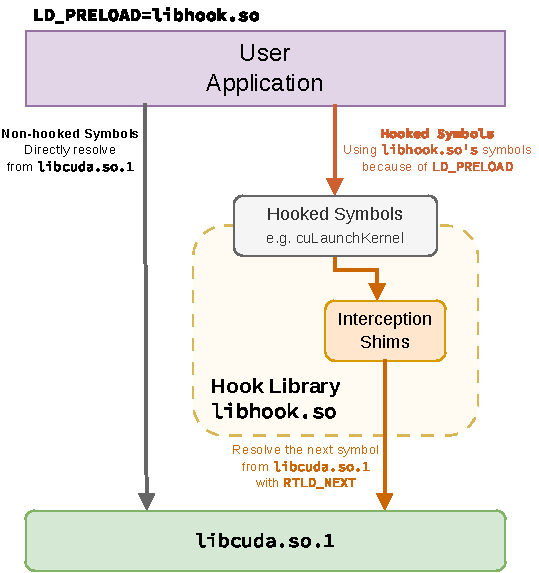
\includegraphics[width=\textwidth]{Figures/Interception_LDPRELOAD.pdf}
        \caption{\texttt{LD\_PRELOAD} interception}
        \label{fig:intercept_ldpreload}
    \end{subfigure}
    \hfill
    \begin{subfigure}{0.49\columnwidth}
        \centering
        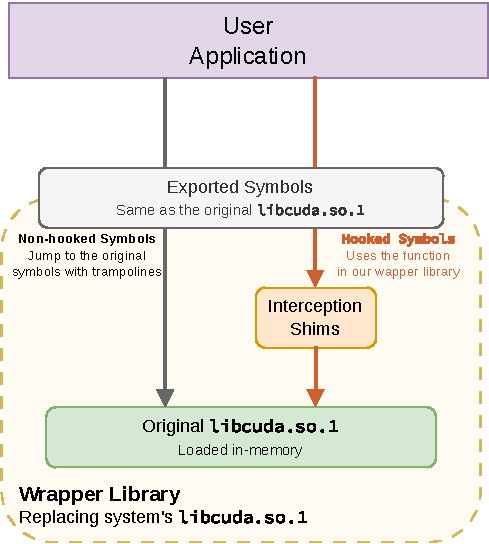
\includegraphics[width=\textwidth]{Figures/Interception_Wrapper.pdf}
        \caption{Wrapper library interception}
        \label{fig:intercept_wrapper}
    \end{subfigure}
    \caption{\texttt{LD\_PRELOAD} interception versus GPU-Sentry's wrapper-library deployment. \texttt{LD\_PRELOAD} requires an additional hook library to be injected ahead of the CUDA driver, while the wrapper replaces the system \texttt{libcuda.so.1} and embeds the original driver.}
    \label{fig:intercept}
\end{figure}

\textbf{Wrapper library.}
Most CUDA Driver API interception tools, including the official CUDA samples~\cite{cuhook-sample-v11.8}, install their hook with \texttt{LD\_PRELOAD} (\cref{fig:intercept_ldpreload}). That mechanism is easy to evade, since a user can simply unset the environment variable, and it is not transparent to containers, because the hook library must also be injected inside each container. GPU-Sentry instead uses a wrapper library (\cref{fig:intercept_wrapper}) that replaces the system \texttt{libcuda.so.1} on the host with its hook, which cannot be disabled by clearing an environment variable. The replacement exposes the expected driver symbols. The original driver library is embedded in the wrapper and extracted and loaded in memory at startup so that intercepted calls can resolve and forward to the real implementation. The wrapper is statically linked and self-contained, so it also runs inside containers: because the NVIDIA Container Toolkit bind-mounts the host's \texttt{libcuda.so.1} into each GPU container, replacing the library once on the host transparently propagates the wrapper to native and containerized workloads alike.

\textbf{Trampoline symbols.}
Symbols that GPU-Sentry does not need to observe are served by trampolines that jump directly to the original implementation with a single \texttt{jmp} instruction. These calls keep the original calling convention and incur only that one jump, so the common CUDA path stays fast.

\textbf{Capturing GPU code objects.}
A CUDA program makes its GPU code available to the device through the module-load and library-load Driver API calls before it can launch any kernel from that code. GPU-Sentry therefore hooks every one of these load paths, listed in the upper block of \cref{tab:hooked_apis}. The captured input may be file-backed or in-memory, and may be a CUBIN, a fatbin, or null-terminated PTX; capture is agnostic to the form, identifying the code type from its magic bytes and reading the object's header to recover its size, which the in-memory load APIs do not provide.

\textbf{Associating kernel-launch handles.}
The kernel-launch Driver API identifies a kernel only by an opaque function handle, not by its name or its code. GPU-Sentry must therefore resolve each handle back to its kernel name and to the module or library that supplied its code. It hooks the handle-resolution and launch entry points in the lower blocks of \cref{tab:hooked_apis}, mapping each function handle to its module or library and thus to the captured code object (\cref{fig:handle}). Each launch event carries process identity, device, stream, function handle, code identifier, launch dimensions, and timestamp.

\begin{table}[t]
    \centering
    \caption{CUDA Driver API entry points intercepted by GPU-Sentry, grouped by role.}
    \label{tab:hooked_apis}
    \begin{tabular}{@{}l p{3.7cm}@{}}
        \toprule
        Driver API & Purpose \\
        \midrule
        \multicolumn{2}{@{}l}{\emph{Code-object load}} \\
        \texttt{cuModuleLoad} & Load a module from a file. \\
        \texttt{cuModuleLoadData} & Load a module from an in-memory image. \\
        \texttt{cuModuleLoadDataEx} & Load a module from memory with JIT options. \\
        \texttt{cuModuleLoadFatBinary} & Load a module from a fat binary. \\
        \texttt{cuLibraryLoadData} & Load a library from an in-memory image. \\
        \texttt{cuLibraryLoadFromFile} & Load a library from a file. \\
        \texttt{cuLibraryGetModule} & Retrieve the code module from a loaded library. \\
        \midrule
        \multicolumn{2}{@{}l}{\emph{Kernel-handle resolution}} \\
        \texttt{cuModuleGetFunction} & Resolve a kernel handle from a module. \\
        \texttt{cuLibraryGetKernel} & Resolve a kernel handle from a library. \\
        \midrule
        \multicolumn{2}{@{}l}{\emph{Kernel launch}} \\
        \texttt{cuLaunchKernel} & Launch a kernel on a stream. \\
        \texttt{cuLaunchKernelEx} & Launch a kernel with extended attributes. \\
        \texttt{cuLaunchCooperativeKernel} & Launch a cooperative kernel. \\
        \bottomrule
    \end{tabular}
\end{table}

\begin{figure}[t]
    \centering
    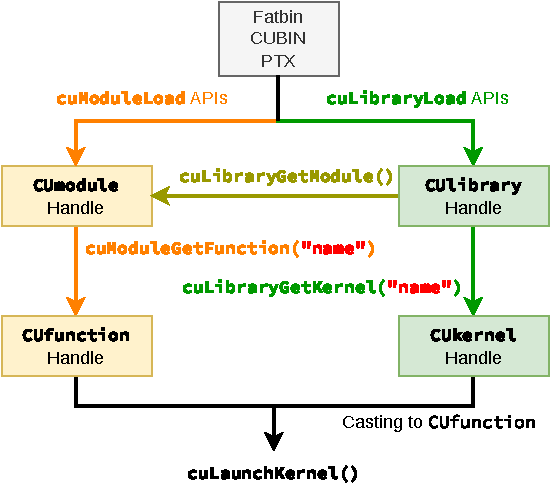
\includegraphics[width=0.82\columnwidth]{Figures/FunctionHandles.pdf}
    \caption{Associating a launched kernel to its SASS. Handle-resolution hooks map a function handle to a module or library, and launch hooks resolve each launch to the captured code object.}
    \label{fig:handle}
\end{figure}

\textbf{Asynchronous buffering.}
The interception path does the minimum work on the application thread: it records a small event holding only the call's metadata, such as handles, identifiers, launch dimensions, and a timestamp, and pushes it into an in-process ring buffer. A background thread batches buffered events and ships them to the collector as Protobuf messages. If the ring buffer fills faster than the background thread can drain it, new events are dropped rather than blocking the application thread, so capture latency stays low even under high launch rates.

\subsection{Kernel Code Normalization Pipeline}
\label{sec:normalization}

GPU-Sentry analyzes SASS, the final representation the device executes: every CUDA program, mining or benign, must ultimately produce SASS to run, whereas higher-level forms such as PTX are optional and can be stripped or absent. Analyzing SASS therefore guarantees coverage of any submitted computation after host compilation, library loading, and PTX JIT translation. Raw SASS, however, is not directly usable for detection: it is specific to a compiler, architecture, and binary instance, and a single kernel often contains regions---initialization, error handling, teardown---that are irrelevant to what it computes. GPU-Sentry therefore passes every captured code object through a normalization pipeline before detection. Code captured as PTX is first compiled to target SASS. Each object is then disassembled~\cite{nvidiaCudaBinaryUtilities}, split into per-kernel instruction sequences, and passed through control-flow analysis: short kernels keep their full normalized sequence, while long kernels are reduced to the main computation loop or compute-heavy section recovered from the control-flow graph, so the classifier focuses on the recurring computational work.

\Cref{alg:mainloop} summarizes the loop selection. GPU-Sentry treats every backward branch---a branch that jumps back to an earlier instruction, the signature of a loop---as the back-edge of a candidate loop, and takes the instructions from the target to the branch as that loop's body. It scores each candidate by a compute weight that rewards the opcode families mining relies on (integer, bitwise, shift, predicate, and memory operations) along with loop size, back-edges, and nesting depth, and keeps the highest-scoring loop. When a kernel has no recoverable loop, it falls back to the whole kernel if the kernel is short, and otherwise to the highest-scoring compute-heavy straight-line region. Because the procedure uses only opcodes and branch targets, it is robust to register allocation and instruction scheduling.

\begin{algorithm}[t]
    \caption{Main computational loop extraction for one kernel.}
    \label{alg:mainloop}
    \begin{algorithmic}[1]
        \REQUIRE normalized instruction list $I$ with branch targets
        \STATE $C \gets \emptyset$ \COMMENT{loop candidates}
        \FORALL{branches $b \in I$ with target $t$ \textbf{before} $b$}
            \STATE $body \gets I[t \mathbin{:} b]$ \COMMENT{back-edge loop body}
            \STATE $C \gets C \cup \{(body,\ \textsc{Score}(body))\}$
        \ENDFOR
        \IF{$C \neq \emptyset$}
            \STATE \textbf{return} body of $\arg\max_{C}\ \textsc{Score}$
        \ELSIF{$|I| \le \tau_{\text{small}}$}
            \STATE \textbf{return} $I$ \COMMENT{short kernel: keep whole body}
        \ELSE
            \STATE \textbf{return} highest-scoring compute-heavy region of $I$
        \ENDIF
        \STATE
        \STATE \textbf{function} \textsc{Score}($body$) \COMMENT{compute weight, higher is more loop-like}
        \STATE \quad \textbf{return} $|body| + \!\!\sum\limits_{f \in \text{families}}\!\! w_f \cdot \mathrm{count}_f(body) + w_{\text{edge}} + w_{\text{nest}}\!\cdot\!\text{depth}$
    \end{algorithmic}
\end{algorithm}

GPU-Sentry normalizes operands to strip unstable details while preserving computation. It canonicalizes instance-specific operands such as registers, addresses, branch labels, and literals, and drops \texttt{NOP} instructions, which carry no computation. It preserves each instruction's opcode and operand types, so the semantic families that matter to both mining and benign compute---integer and bitwise arithmetic, memory access, control flow, and floating-point or tensor math---remain distinguishable. \Cref{lst:normalization} shows the effect.

\begin{lstlisting}[caption={SASS normalization preserves opcode and operand-type semantics while removing instance-specific detail.},label={lst:normalization}]
IADD3 R12, R13, c[0x0][0x20], RZ
  -> IADD3 REG, REG, CONST, ZERO

@P0 BRA 0x1a0
  -> @PRED BRA LABEL
\end{lstlisting}

GPU-Sentry also maps architecture-specific opcode variants to common semantic families, because GPU generations often express the same operation with different opcodes or qualifiers. Integer multiply-add, for instance, is \texttt{XMAD} on Maxwell and Pascal but \texttt{IMAD} on Volta and later, and both map to \texttt{IMAD}; a warp shuffle is \texttt{SHFL} before Volta and \texttt{SHFL.SYNC} from Volta onward, and both map to \texttt{SHFL}. This keeps semantically equivalent integer, bitwise, memory, branch, and synchronization patterns comparable across compilers and GPU generations.

\subsection{Dynamic Kernel-Launch Window Scheduler}
\label{sec:windows}

A mining workload is usually a launch \emph{sequence}, not a single isolated kernel: a miner launches its kernels repeatedly, and many mining algorithms spread their work across several distinct kernels. GPU-Sentry therefore analyzes streams of launches. It maintains a per-stream rolling window, grouping launches by process, device, and CUDA stream. Grouping by stream both preserves CUDA launch order within a workload and keeps unrelated work apart, so the repeated or split launches of one miner accumulate in the same window while every verdict stays attributable to one process. The detector consumes one fixed-size sequence at a time, so the scheduler's job is to turn an unbounded launch stream into model-sized windows, each rendered to the content budget of 8190 tokens (reserving two of the model's 8192 positions for the \texttt{[CLS]} and \texttt{[SEP]} tokens).

\Cref{alg:scheduler} summarizes the per-stream window-scheduling logic; the paragraphs below explain its parts.

\begin{algorithm}[t]
    \caption{Per-stream window scheduler, run on each kernel launch.}
    \label{alg:scheduler}
    \begin{algorithmic}[1]
        \REQUIRE \parbox[t]{0.86\linewidth}{per-stream state:\\
            \hspace*{1em}$W$: launch window, oldest to newest;\\
            \hspace*{1em}$c$: total token cost currently in $W$;\\
            \hspace*{1em}$M$: multiset of live kernel ids in $W$;\\
            \hspace*{1em}$S$: composition signatures already emitted for the stream;\\
            \hspace*{1em}$B = 8190$: content-token budget}
        \STATE \textbf{On kernel launch} $k$ \textbf{on its stream:}
        \STATE append $k$ to $W$;\ \ $c \gets c + \textsc{TokenCost}(k)$;\ \ increment $M[k.\textit{id}]$
        \IF{$c \le B$}
            \RETURN \COMMENT{budget not full; keep collecting}
        \ENDIF
        \STATE $\sigma \gets \langle \textsc{SortedSet}(M),\ \textsc{Top3}(M) \rangle$ \COMMENT{composition signature}
        \IF{$\sigma \notin S$}
            \STATE \textbf{emit} \textsc{Render}($W$) as one window \COMMENT{composition not classified for the stream yet}
            \STATE $S \gets S \cup \{\sigma\}$
        \ENDIF
        \WHILE{$c > B$}
            \STATE pop oldest launch $k_0$ from $W$;\ \ $c \gets c - \textsc{TokenCost}(k_0)$;\ \ decrement $M[k_0.\textit{id}]$
        \ENDWHILE
        \STATE
        \STATE \textbf{function} \textsc{Render}($W$) \COMMENT{turn the window into one ModernBERT input}
        \STATE \quad $r \gets$ concat normalized kernels in $W$, joined by \texttt{KERNEL\_BOUNDARY}
        \STATE \quad \textbf{return} \textsc{KeepLast}($r$, $B$) \COMMENT{clip to $B$ tokens, keep the newest}
    \end{algorithmic}
\end{algorithm}

\textbf{Filling and emitting a window.}
Each launch contributes a known token cost: its rendered normalized SASS fragment plus one \texttt{KERNEL\_BOUNDARY} token. GPU-Sentry appends each launch to the stream's window and accumulates its cost, collecting launches until the window fills the token budget. It then emits the full window for classification and evicts the oldest launches to make room for the next one. Waiting until the budget is full ensures every emitted window carries enough code to classify, rather than a tiny first-launch fragment.

\textbf{Composition-signature deduplication.}
A steady stream fills and emits windows repeatedly with the same kernel mixture, so GPU-Sentry deduplicates emissions by composition signature: the sorted set of live kernel identities together with the three most frequent kernels. A window is emitted only if its signature has not been emitted before for that stream, so a stream is classified when its kernel composition is new rather than on every full window.

\textbf{Rendering and front clipping.}
The \textsc{Render} subroutine in \cref{alg:scheduler} turns a window into one ModernBERT input: it concatenates the window's normalized launch fragments joined by \texttt{KERNEL\_BOUNDARY} tokens, and because a full window can slightly exceed the budget, clips from the front and keeps the newest fragments so the final input is exactly one model-sized sequence. The scheduler therefore owns the token budget and the detector classifies exactly one sequence per window. \Cref{lst:window} shows a rendered window.

\begin{lstlisting}[caption={A rendered window concatenates per-launch normalized SASS fragments, separated by \texttt{KERNEL\_BOUNDARY} tokens, into one model-sized sequence.},label={lst:window}]
; Normalized main loop for Kernel 1
IADD3 REG, REG, CONST, ZERO
LOP3 REG, REG, REG, CONST
SHF REG, REG, IMM
@PRED BRA LABEL
KERNEL_BOUNDARY
; Normalized main loop for Kernel 2
IMAD REG, REG, REG, ZERO
LDG REG, MEM
STG MEM, REG
KERNEL_BOUNDARY
...
\end{lstlisting}

\subsection{ModernBERT Instruction-Sequence Detector}
\label{sec:classifier}

GPU-Sentry classifies each normalized instruction window with a learned model: an encoder-only ModernBERT model~\cite{warner2024modernbert} used as a binary classifier over normalized instruction sequences. Because it is encoder-only, it attends over the whole token window at once, which makes it a fast detector and lets it learn both local instruction relationships within a kernel and recurrence patterns across launches. We use an encoder rather than a decoder-only LLM because detection is a classification task that needs no left-to-right text generation, which keeps inference cheaper for the same context length. Its input is normalized SASS joined by \texttt{KERNEL\_BOUNDARY} tokens; scheduling metadata such as timestamps, launch dimensions, and process names are deliberately excluded so the model reasons about code, not context.

Because the scheduler already bounds every window to the content budget, each rendered window yields a single mining probability. A per-window threshold gives a diagnostic verdict, while the deployment decision is made by the workload policy below. ModernBERT is the primary and sole decision layer in this work (\cref{sec:evaluation}).

\subsection{Decision}
\label{sec:decision}

The decision module separates detection output from deployment policy. Each classified window yields a mining score and the capture context needed for attribution, but a single window may not carry enough evidence for a confident decision, so GPU-Sentry aggregates per-window scores into a workload decision with a rolling policy over the most recent windows of a stream (the last eight in our deployment). A workload is flagged when the rolling mean mining probability is at least 0.30 \emph{and} the rolling maximum is at least 0.50 (\cref{sec:thresholds} describes how both thresholds are chosen). The mean term requires sustained mining-like evidence across the workload, while the max term keeps a benign workload with many steady, moderate scores from triggering on its average alone. When the policy fires, a deployment may notify an administrator through a notification channel or block the workload by sending a termination command to the client interception thread, on receipt of which the offending process self-terminates.

\subsection{Archive}
\label{sec:archive}

GPU-Sentry archives captured code objects, normalized artifacts, window metadata, model scores, and verdicts to disk. Unlike device telemetry, which can only show that the GPU was busy, instruction-level detection produces evidence that can be re-examined after an alert.

\subsection{Implementation}
\label{sec:implementation}

The interception library is implemented in C++ together with a Go client bridge that exports events on a background thread; the two are statically linked into a single replacement \texttt{libcuda.so.1}. Events are serialized as Protobuf and sent to the collector over UDP. The collector server is implemented in Go, and offline analysis and ModernBERT training run in Python. The same capture path is used both to build datasets and to run deployment-mode experiments.

\subsection{Extensibility: Optional Verification Layer}
\label{sec:verifier}

For deployments with stricter false-positive tolerance, GPU-Sentry can route uncertain windows to an optional second-stage verifier, for example a locally hosted LLM, that reasons jointly over the un-normalized main-loop code, kernel statistics, ModernBERT scores, and launch behavior, explicitly weighing benign crypto-like alternatives such as cryptographic libraries, compression, checksums, password-recovery benchmarks, and integer-heavy HPC. This layer is conceptual and unimplemented in this work: we report results from ModernBERT alone, so the verifier is never invoked in our experiments. It targets exactly the low-confidence borderline cases the detector currently mishandles, such as the single-window captures missed in our real-world evaluation, and we leave its implementation and evaluation to future work.

\section{Dataset and Training}
\label{sec:dataset}

\subsection{Synthetic-to-Real Transfer}

Real GPU-miner datasets are too small to train a detector on directly and too difficult to collect at scale, so GPU-Sentry adopts a synthetic-to-real protocol: it learns from synthetic normalized SASS and is evaluated on real captures, which tests transferable instruction-level patterns rather than memorization. The tokenizer, the masked-language model, and the classifier are all trained and selected only on synthetic data; no real-world capture is used to train, validate, or select the learned detector, so the real-world dataset is evaluation-only. Only the workload policy's two decision thresholds are set on the real-world distributions as deployment operating points (\cref{sec:thresholds}); the learned model itself never sees real data.

\subsection{Synthetic Workloads}

The synthetic dataset contains 252 captured workloads, evenly split across O2 and O3 builds, with 130 mining-like and 122 benign workloads. The workloads were generated from algorithm lists and natural-language descriptions and implemented with the assistance of a large language model (GPT-5.5~\cite{openai_gpt55}), and each algorithm is built both as a single-kernel (mono) variant and as a split variant that distributes work across helper kernels, so the detector sees both compact and split execution. \Cref{tab:synthetic_dataset} lists representative algorithms in each class together with the workload counts. Because the scheduler can emit more than one window per workload, the 252 workloads yield 361 windows under a grouped 70/15/15 split (253 train, 56 validation, 52 test), with all windows of a workload kept on the same side of the split.

\begin{table}[t]
    \centering
    \caption{Synthetic normalized-SASS dataset used for training and synthetic validation/testing, with representative algorithms per class. Counts are total workloads (train / val / test).}
    \label{tab:synthetic_dataset}
    \footnotesize
    \begin{tabular}{@{}l p{4.4cm} r@{}}
        \toprule
        Class & Representative algorithms & Total (tr/va/te) \\
        \midrule
        Mining & Ethash, Etchash, ProgPoW, KawPoW, FiroPoW, CryptoNight, RandomX, Cuckaroo29, Cuckatoo31, Equihash, BeamHash~III, Autolykos2, MTP, Octopus, Verthash, X16R, GhostRider, FishHash, KarlsenHash~v2, kHeavyHash, SHA-256d, Blake3, Keccak & 130 (91/20/19) \\
        \midrule
        Benign compute & SGEMM/DGEMM, Conv2D, attention, softmax, LayerNorm, FFT, DCT, Sobel, PageRank, BFS, SSSP, bitonic sort, prefix scan, reduction, Huffman, LZ match, CRC32, xxHash & 80 (56/12/12) \\
        \midrule
        Benign crypto & SHA-256, SHA-512, Keccak, BLAKE2b, ChaCha20, AES, Merkle tree, Philox RNG & 28 (20/4/4) \\
        \midrule
        Benign memory & STREAM copy/scale/add/triad, pointer chase, gather/scatter, random-index read & 14 (10/2/2) \\
        \midrule
        \textbf{Total} & & \textbf{252 (177/38/37)} \\
        \bottomrule
    \end{tabular}
\end{table}

The benign crypto/hash-like class is included deliberately as a hard negative. Cryptographic primitives and checksums can be dominated by the same integer and bitwise instructions that characterize proof-of-work hashing, so this class probes whether the detector has learned more than a naive ``bitwise-heavy means mining'' association.

\textbf{Split policy.}
The synthetic train, validation, and test splits avoid leakage from shared lineage. Workloads that share a source algorithm, implementation, or binary are kept on the same side of a split rather than divided at random, and the O2 and O3 variants of a workload are kept together, so the model cannot trivially match a window to its optimization twin across splits.

\subsection{Real-World Captures}

The real-world dataset is collected through the same runtime capture layer used in deployment, and we build it into 58 evaluation-only workload groups: 48 mining-like and 10 benign. The mining captures come from production GPU miners and the benign captures from real GPU applications. Because some miners support many algorithms, we run each miner once per algorithm and treat each (miner, algorithm) run as a separate workload. \Cref{tab:realworld_programs} lists the captured programs and group counts.

\begin{table}[t]
    \centering
    \caption{Real-world evaluation dataset: captured programs and workload-group counts. Miners are captured per algorithm; all groups are evaluation-only.}
    \label{tab:realworld_programs}
    \begin{tabular}{@{}l p{5.0cm} r@{}}
        \toprule
        Type & Programs (example algorithms) & Groups \\
        \midrule
        Miners & T-Rex, GMiner, lolMiner, NBMiner, Rigel, XMRig \newline (ethash, etchash, kawpow, progpow, octopus, autolykos2, kheavyhash, randomx) & 48 \\
        \midrule
        Benign apps & PyTorch training, vLLM inference, HPL, Blender OptiX, cuBLAS GEMM, cuDNN convolution, GPU compression, CRC32 / SHA-256 / AES benchmarks & 10 \\
        \midrule
        \textbf{Total} & & \textbf{58} \\
        \bottomrule
    \end{tabular}
\end{table}

\subsection{ModernBERT Training}

The detector is a compact encoder-only ModernBERT: 8 transformer layers, hidden size 384, 6 attention heads, and a maximum sequence length of 8192 tokens. Its inputs are normalized SASS, so a small word-level tokenizer with a 64-token vocabulary suffices. Training proceeds in three stages on the synthetic data. GPU-Sentry first trains the tokenizer on normalized SASS from the training split, then warms the model from scratch with masked-language modeling (8 epochs, 15\% masking) to learn instruction semantics, and finally trains the binary classifier (10 epochs). \Cref{tab:training} summarizes the configuration.

\begin{table}[t]
    \centering
    \caption{ModernBERT detector configuration.}
    \label{tab:training}
    \small
    \begin{tabular}{@{}ll@{}}
        \toprule
        Item & Value \\
        \midrule
        Architecture & encoder-only, 8 layers, hidden 384, 6 heads \\
        Max sequence length & 8192 tokens \\
        Tokenizer & word-level SASS, vocabulary 64 \\
        MLM pretraining & 8 epochs, 15\% masking, eval loss 0.083 \\
        Classifier training & 10 epochs, binary \\
        \bottomrule
    \end{tabular}
\end{table}

On the held-out synthetic windows the detector is perfect (\cref{tab:synthetic_results}): window-level accuracy and macro F1 are 1.000 on both validation (56 windows) and test (52 windows), and aggregating windows to workloads is likewise perfect on validation, test, and the two combined. This clean synthetic fit, together with the hard-negative crypto class, is what makes the real-world captures the meaningful test of transfer (\cref{sec:evaluation}).

\begin{table}[t]
    \centering
    \caption{Binary detector results on the synthetic validation and test splits (window-level). Workload-level aggregation is also 1.000 on both splits.}
    \label{tab:synthetic_results}
    \small
    \begin{tabular}{lrrr}
        \toprule
        Split & Windows & Acc. & Macro F1 \\
        \midrule
        Validation & 56 & 1.000 & 1.000 \\
        Test & 52 & 1.000 & 1.000 \\
        \bottomrule
    \end{tabular}
\end{table}

\section{Evaluation}
\label{sec:evaluation}

Our evaluation asks four questions: whether GPU-Sentry captures representative CUDA activity at low overhead, whether synthetic training transfers to real-world SASS windows, whether instruction-level detection resists launch-rate throttling, and whether per-stream windows survive mixed workloads, in each case compared against a telemetry baseline.

\subsection{Experimental Setup}

Experiments run on a server with two Intel Xeon Silver 4314 CPUs, 188\,GiB RAM, and eight NVIDIA V100 GPUs, on Debian 12 with Linux 6.1.0, NVIDIA driver 580.65.06, and CUDA 12.8.

\textbf{Baseline.}
We compare against a behavioral baseline drawn from Pott-style GPU-counter detection~\cite{pott2023gpucryptojacking}: a Random Forest over whole-device NVML~\cite{nvidiaNvml} point measurements (GPU utilization, memory utilization, power, and temperature). It predicts a mining probability per sample and raises a run-level alarm when the mean mining probability is at least 0.8, a threshold tuned on its own validation split with a maximum benign false-positive rate of 0.01. We restrict the comparison to detectors that, like GPU-Sentry, reason about GPU execution; network, host-signature, and side-channel detectors target a different signal and are out of scope here.

\subsection{Capture Effectiveness}

GPU-Sentry must first show that transparent capture observes real CUDA activity across benign and mining workloads. \Cref{tab:top_kernels} reports the three most frequently launched named kernels in representative vLLM, HPL, and T-Rex captures, each chosen to stress a different capture path: vLLM runs on the PyTorch framework, HPL (the NVIDIA HPC Benchmarks 21.4 image from NGC) runs inside a Docker container, and T-Rex uses biinary obfuscation and anti-debugging techniques. GPU-Sentry captures AI serving kernels, dense linear algebra kernels, and mining search kernels through the same Driver-API path. The HPL case shows that capture reaches containerized workloads, and the T-Rex case is the important one for evasion: even though T-Rex obfuscates its host process, its GPU computation must still traverse the Driver API, so GPU-Sentry captures its \texttt{cuda\_ethash\_search} kernels and their SASS.

\begin{table*}[t]
    \centering
    \caption{Top launched named kernels from representative captures, each exercising a different capture challenge. Compute ratio is the fraction of parsed SASS instructions in compute opcode families.}
    \label{tab:top_kernels}
    \begin{tabular}{lllrrr}
        \toprule
        Workload & Capture challenge & Kernel & Launches/s & Instr. & Compute ratio \\
        \midrule
        \multirow{3}{*}{vLLM} & \multirow{3}{*}{PyTorch framework} & \texttt{reshape\_and\_cache\_kernel\_flash} & 132.758 & 50 & 0.680 \\
         & & \texttt{triton\_red\_fused\_...} & 127.371 & 158 & 0.753 \\
         & & \texttt{triton\_poi\_fused\_...} & 127.320 & 143 & 0.881 \\
        \midrule
        \multirow{3}{*}{HPL} & \multirow{3}{*}{Containerized} & \texttt{volta\_dgemm\_128x64\_nt} & 42.471 & 1054 & 0.793 \\
         & & \texttt{trsm\_right\_kernel<\dots,true>} & 41.683 & 198 & 0.576 \\
         & & \texttt{trsm\_right\_kernel<\dots,false>} & 41.683 & 184 & 0.516 \\
        \midrule
        \multirow{3}{*}{T-Rex} & \multirow{3}{*}{Obfuscation \& anti-debug} & \texttt{cuda\_ethash\_search} & 57.796 & 1512 & 0.854 \\
         & & \texttt{cuda\_ethash\_search\_1} & 29.190 & 1555 & 0.849 \\
         & & \texttt{cuda\_ethash\_search\_2} & 29.044 & 2088 & 0.800 \\
        \bottomrule
    \end{tabular}
\end{table*}


\subsection{Capture Overhead}

GPU-Sentry adds a small latency to CUDA Driver-API calls (\cref{tab:api_overhead}, medians over 100 runs of a vector-add program). The jump-only \texttt{cuDeviceGetCount} trampoline adds about 0.13\,$\mu$s, module load adds about 68.7\,$\mu$s because GPU-Sentry records the loaded code object, and kernel launch adds about 9.8\,$\mu$s. Asynchronous buffering is what keeps the launch path cheap. We compare against our previous capture system, cuPCAP~\cite{kuo2025cupcap}, which exports each event synchronously on the intercept path and, lacking trampolines, wraps every forwarded call in an extra stack frame: it adds about 16.0\,$\mu$s per launch, so GPU-Sentry's in-process ring buffer cuts kernel-launch overhead by roughly 40\% (9.8 versus 16.0\,$\mu$s). The same asynchrony keeps module-load and trampoline latency far below the synchronous design across all three calls.

\begin{table}[t]
    \centering
    \caption{Median CUDA Driver-API latency ($\mu$s): native, our prior synchronous capture design cuPCAP, and GPU-Sentry's asynchronous capture; parentheses give the latency added over native. Asynchronous buffering lowers the added latency, most importantly for kernel launch.}
    \label{tab:api_overhead}
    \footnotesize
    \begin{tabular}{lrrr}
        \toprule
        API call & Native & cuPCAP (sync) & GPU-Sentry (async) \\
        \midrule
        \texttt{cuDeviceGetCount} & 2.575 & 6.545 (+3.970) & 2.706 (+0.131) \\
        \texttt{cuModuleLoad} & 133.819 & 402.839 (+269.020) & 202.484 (+68.665) \\
        \texttt{cuLaunchKernel} & 25.302 & 41.292 (+15.990) & 35.081 (+9.780) \\
        \bottomrule
    \end{tabular}
\end{table}

At the application level, the overhead is not measurable for the representative workloads (\cref{tab:app_overhead}). HPL reports 3608 GFLOP/s without capture and 3721 GFLOP/s with capture, within run-to-run variation; T-Rex reports an identical 90.75 MH/s; and vLLM reports 1827.68 versus 1827.91 tokens/s. Because module loads are rare relative to kernel launches and launches are buffered asynchronously, capture stays off the throughput-critical path.

\begin{table}[t]
    \centering
    \caption{Application throughput with and without capture. Overhead is the relative throughput loss $(\mathrm{native}-\mathrm{capture})/\mathrm{native}$; negative values mean capture measured slightly faster, within run-to-run variation.}
    \label{tab:app_overhead}
    \begin{tabular}{llrrr}
        \toprule
        Workload & Metric & Native & Capture & Overhead (\%) \\
        \midrule
        HPL & GFLOP/s & 3608 & 3721 & $-3.1$ \\
        T-Rex & MH/s & 90.75 & 90.75 & $0.0$ \\
        vLLM & tokens/s & 1827.68 & 1827.91 & $-0.01$ \\
        \bottomrule
    \end{tabular}
\end{table}

\subsection{Synthetic-to-Real Detection}

Because the learned detector is trained only on synthetic data, we evaluate it on all 58 real-world workload groups, applying the same rolling workload policy used online (\cref{sec:decision}). This yields the confusion matrix in \cref{tab:realworld_detection} and the metrics in \cref{tab:realworld_metrics}: GPU-Sentry reaches 0.966 accuracy and 0.944 macro F1, flagging 46 of 48 mining workloads (0.958 recall) with no benign false positives (1.000 mining precision, 1.000 benign recall). The two missed workloads are the Pyrin-family miners \texttt{lolminer\_pyrin} and \texttt{lolminer\_pyrinv2}, whose matrix-hash code the detector scores as benign (mining probability 0.027 and 0.100); we analyze this representation limit, which no threshold can fix, in \cref{sec:thresholds}.

\begin{table}[t]
    \centering
    \caption{Real-world workload-level detection for GPU-Sentry over all 58 workload groups under the rolling workload policy. Rows are ground truth, columns are predictions.}
    \label{tab:realworld_detection}
    \begin{tabular}{lrr}
        \toprule
        True label & Pred. benign & Pred. mining \\
        \midrule
        Benign & 10 & 0 \\
        Mining & 2 & 46 \\
        \bottomrule
    \end{tabular}
\end{table}

\begin{table}[t]
    \centering
    \caption{Real-world workload-level detection metrics over all 58 workload groups.}
    \label{tab:realworld_metrics}
    \begin{tabular}{lrrrr}
        \toprule
        Class & Workloads & Precision & Recall & F1 \\
        \midrule
        Benign & 10 & 0.833 & 1.000 & 0.909 \\
        Mining & 48 & 1.000 & 0.958 & 0.979 \\
        \midrule
        \multicolumn{1}{l}{Accuracy} & \multicolumn{4}{r}{0.966 (56/58)} \\
        \multicolumn{1}{l}{Macro F1} & \multicolumn{4}{r}{0.944} \\
        \bottomrule
    \end{tabular}
\end{table}

The benign side is clean because the detector scores benign workloads low and the workload policy requires sustained, high-confidence evidence: every benign application, including compute-bound ones such as cuBLAS GEMM, cuDNN convolution, HPL, and Blender OptiX, stays below the policy thresholds (\cref{sec:thresholds}).

\textbf{Comparison with the behavioral baseline on basic runs.}
The behavioral baseline is just as accurate on these ordinary isolated runs, which is why telemetry detectors are attractive in practice. We score the same real-world workloads with the synthetic-trained Random Forest under the same synthetic-to-real transfer, replaying each workload under whole-device telemetry capture without retraining. On this set of 48 mining and 10 benign workloads the baseline reaches 0.979 mining recall with no benign false positives (\cref{tab:basic_compare,tab:baseline_confusion}), level with GPU-Sentry's 0.958 from \cref{tab:realworld_metrics}. Both detectors are therefore strong on ordinary runs; the contrast emerges only under launch-rate throttling and mixed workloads (\cref{fig:throttle,tab:mixed}), where the baseline collapses while GPU-Sentry stays at 1.000. The two detectors also fail on different axes: the baseline's single miss is the RandomX miner \texttt{xmrig}, whereas GPU-Sentry's are the Pyrin-family matrix-hash miners.

\begin{table}[t]
    \centering
    \caption{Basic-run detection on the same real-world isolated workloads (48 mining, 10 benign). Both detectors are accurate on ordinary runs; the gap appears only under throttling and mixed workloads. The behavioral baseline replays each workload under telemetry and scores it with the synthetic-trained Random Forest; the GPU-Sentry row repeats \cref{tab:realworld_metrics} for side-by-side comparison.}
    \label{tab:basic_compare}
    \begin{tabular}{lrrr}
        \toprule
        Detector & Mining recall & Benign recall & Accuracy \\
        \midrule
        Behavioral baseline & 0.979 (47/48) & 1.000 (10/10) & 0.983 (57/58) \\
        \textbf{GPU-Sentry} & 0.958 (46/48) & 1.000 (10/10) & 0.966 (56/58) \\
        \bottomrule
    \end{tabular}
\end{table}

\begin{table}[t]
    \centering
    \caption{Behavioral baseline confusion matrix on the real-world isolated workloads (10 benign, 48 mining). Rows are ground truth, columns are predictions.}
    \label{tab:baseline_confusion}
    \begin{tabular}{lrr}
        \toprule
        True label & Pred. benign & Pred. mining \\
        \midrule
        Benign & 10 & 0 \\
        Mining & 1 & 47 \\
        \bottomrule
    \end{tabular}
\end{table}

\subsection{Threshold Selection}
\label{sec:thresholds}

GPU-Sentry's only tuned decision point is the rolling workload policy (\cref{sec:decision}): the learned detector is trained and selected on synthetic data, while the policy's two scalar thresholds are chosen from the real-world workload distributions in \cref{fig:decision_threshold}.

The workload policy flags a stream only when its rolling mean mining probability is at least 0.30 \emph{and} its rolling maximum is at least 0.50. \Cref{fig:decision_threshold} plots each real-world workload's mean and maximum mining probability. No benign workload enters the flagged region. A maximum-only rule would fail: three benign workloads (vLLM, AES, and compression) each contain a single window the model scores above 0.93, which it would flag as mining. The mean term is what rejects these false positives: averaged over each workload's many other low-scoring windows, their rolling mean stays below 0.23, well under the 0.30 threshold. A mean-only rule, conversely, would miss borderline miners whose evidence is concentrated in a few windows, so the maximum term keeps them flagged. The only two mining workloads that fall outside the flagged region, near the origin, are \texttt{lolminer\_pyrin} and \texttt{lolminer\_pyrinv2}; their low scores are a fundamental representation limit rather than a threshold artifact, discussed below.

\begin{figure}[t]
    \centering
    \includesvg[width=\columnwidth]{Figures/decision_threshold}
    \caption{Per-workload mean versus maximum mining probability on the real-world set. The flagged region (shaded) requires mean $\geq 0.30$ and max $\geq 0.50$. Benign workloads with one spiky window sit top-left (high max, low mean) and are excluded by the mean term; no benign workload is flagged. The two Pyrin-family miners near the origin are scored benign by the detector because their matrix-hash SASS resembles AI matmul.}
    \label{fig:decision_threshold}
\end{figure}

\textbf{The Pyrin matrix-hash case.}
The two missed miners, \texttt{lolminer\_pyrin} and \texttt{lolminer\_pyrinv2}, are not threshold failures: their mean and maximum mining probabilities are 0.027 and 0.100, far below any usable threshold. Pyrin's proof-of-work is a matrix-multiplication hash deliberately designed to be ASIC-resistant by mapping the hash onto the same dense integer matrix-multiply primitives that GPUs and AI accelerators are built for. The resulting SASS is dominated by integer dot-product (\texttt{IDP}) instructions and is, at the instruction level, essentially indistinguishable from a benign integer-GEMM or quantized-inference kernel. This is an inherent limit of code-level detection for matmul-style mining algorithms, not a tuning choice, and it motivates the optional verification layer and runtime-context signals (\cref{sec:verifier}).

\subsection{Launch-Rate Throttling}

Throttling the kernel-launch loop affects telemetry far more than instruction-level detection (\cref{fig:throttle}). GPU-Sentry evaluates 288 windows from throttled captures across all synthetic mining algorithms, at 10\%, 50\%, 75\%, and 100\% launch rates, and classifies all 288 as mining (recall 1.000 at every rate). Throttling changes launch timing, not the normalized SASS body or the token cost each launch contributes, so a throttled stream still fills the budget and the emitted window still contains the mining kernels; it just fills more slowly.

\begin{figure}[t]
    \centering
    \includesvg[width=\columnwidth]{Figures/throttle}
    \caption{Mining recall versus kernel-launch throttling. GPU-Sentry stays at 1.000 across the evaluated rates (5--100\%), while the GPU-counter behavioral baseline collapses to 0 at mid rates (25--75\%) and recovers only at the 5\% and 100\% extremes. Aggregated, GPU-Sentry detects 288/288 windows (recall 1.000) and the baseline 23/48 runs (recall 0.479).}
    \label{fig:throttle}
\end{figure}

The behavioral baseline detects every run at the 5\% and 100\% settings but misses every run at 25\%, 50\%, and 75\% and one of eight at 10\%. Mid-rate throttling moves utilization and power into ordinary-looking bands where the device counters no longer look mining-like. The 5\% and 100\% recoveries have opposite causes. At 100\% the device shows its native full-rate mining footprint, which the baseline learned as mining. At the 5--10\% extreme, by contrast, heavy throttling collapses the footprint to a near-idle range ($\approx$5--10\% utilization, $\approx$40\,W) that lies outside the busy benign workloads the Random Forest was trained on; the classifier therefore flags these runs as ``not a heavy benign job'' with high confidence rather than recognizing mining as such. This is brittle: the same boundary would raise false alarms on any genuinely idle or lightly loaded GPU, so it is not the robustness it appears to be. The mid rates instead place the device squarely in the ordinary busy-workload band that overlaps benign jobs, where confidence collapses and the alarm never fires. This is the sharpest contrast between the two approaches: GPU-Sentry is invariant to launch-rate throttling because it reads the kernel body.

\subsection{Mixed Workloads}

When a benign workload and a throttled miner share one GPU, whole-device telemetry loses the miner, but instruction-level detection does not. We co-locate each of seven mining algorithms with a representative benign GPU workload on one device (\cref{tab:mixed}). The behavioral baseline detects only two of the seven, because the benign workload dominates the shared device counters. It also has no PID or stream attribution, so even when it does alarm it cannot point to the offending process. GPU-Sentry detects all seven mining streams. Its windows are per process and per stream by construction, so the benign stream and the mining stream remain separate detection units: the mining stream emits the same normalized SASS window it would emit on its own, regardless of the co-running benign job, and the detector classifies it independently and attributes it to the offending PID and stream. Sharing the device therefore changes neither the kernel body nor GPU-Sentry's decision, which is why mixing leaves its recall unchanged while it collapses the telemetry baseline.

\begin{table}[t]
    \centering
    \caption{Mixed-workload runs. Each run co-locates a benign GPU workload with a throttled miner on one device. Whole-device counters miss most miners and cannot attribute alarms to a process; GPU-Sentry's per-stream windows isolate and detect every mining stream. The cuBLAS GEMM run was repeated, for seven runs total.}
    \label{tab:mixed}
    \small
    \begin{tabular}{llcc}
        \toprule
        Benign co-tenant & Miner & Behavioral baseline & GPU-Sentry \\
        \midrule
        cuBLAS GEMM & RandomX & $\times$ & $\checkmark$ \\
        cuDNN convolution & KawPoW & $\times$ & $\checkmark$ \\
        HPL (Linpack) & SHA-256d & $\times$ & $\checkmark$ \\
        PyTorch training & Ethash & $\checkmark$ & $\checkmark$ \\
        AES & Ethash & $\times$ & $\checkmark$ \\
        vLLM inference & RandomX & $\checkmark$ & $\checkmark$ \\
        \midrule
        \multicolumn{2}{l}{Mining recall} & 0.286 (2/7) & \textbf{1.000 (7/7)} \\
        \bottomrule
    \end{tabular}
\end{table}


\section{Limitations}
\label{sec:limitations}

\textbf{Userspace enforcement boundary.} GPU-Sentry's main deployment limitation is that it runs in a userspace library, so a same-privilege user can bypass it---by shipping their own \texttt{libcuda.so.1}, calling the driver directly, or tampering with the monitored library. Moving the check into the kernel does not work either: once a program has a GPU channel, it submits each launch by writing directly to a command buffer that the kernel never sees. The kernel does still hand out those channels in the first place, so NVIDIA's open-source GPU kernel modules make enforcement possible: an administrator could allow a GPU channel to be created only through the monitored path, leaving a user no way to obtain an unmonitored one. We leave this to future work.

\textbf{Code obfuscation.} Obfuscation can also weaken instruction-level detection by changing the instruction stream enough to hide mining-like structure. On a GPU this is unusually costly: a mining kernel is the workload's core computation, hand-tuned for throughput through register allocation, occupancy, memory-access patterns, and instruction scheduling, so inserting instructions or perturbing its control flow degrades exactly the performance the miner depends on. Because mining revenue scales with hash throughput, obfuscation trades away profit, and no GPU-code obfuscation tooling exists for this purpose today. GPU-Sentry does not assume obfuscation is impossible; it treats obfuscated or low-confidence cases as a reason for additional verification and audit rather than as solved.

\textbf{Benign-looking mining algorithms.} The sharpest limit is a proof-of-work that is, by construction, the same computation as a benign GPU kernel. Matrix-multiplication proof-of-work such as Pyrin is designed to be ASIC-resistant by mapping the hash onto the same dense integer matrix-multiply primitives that GPUs and AI accelerators are optimized for, so its SASS is essentially indistinguishable from benign integer GEMM or quantized inference (\cref{sec:thresholds}). Code-level detection alone cannot separate such workloads from legitimate AI compute; distinguishing them requires runtime context or a second-stage verifier (\cref{sec:verifier}) rather than the instruction window alone.

\section{Related Work}
\label{sec:related}

\textbf{GPU cryptojacking detection.}
Prior GPU cryptojacking detectors reason about behavior, telemetry, or counters: decision trees over host and GPU metrics~\cite{tanana2024gpucryptojacking}, classifiers over GPU device telemetry~\cite{pott2023gpucryptojacking}, and physical side-channel monitors~\cite{xiao2023magtracer,cao2025maginspector}. These methods are practical because they need no code inspection, but they infer intent from effects such as utilization, power, repeated launches, or counter patterns, which we show degrade under throttling and mixed workloads. GPU-Sentry instead captures and classifies the submitted GPU instruction stream; to our knowledge, it is the first GPU-cryptomining detector to use the submitted GPU instructions (SASS) as its detection signal rather than these indirect effects.

\textbf{GPU binary instrumentation and capture.}
GPU binary instrumentation frameworks such as NVBit~\cite{villa2019nvbit} and SASSI~\cite{stephenson2015sassi} can observe execution at instruction granularity, and observability tools such as DCGM, Nsight Systems, and CUPTI expose rich runtime signals~\cite{dcgm,nsight-systems,cutpi}. These tools target profiling, debugging, and cluster monitoring rather than deciding whether a SASS window implements mining, and per-instruction instrumentation is heavier than continuous monitoring needs. GPU-Sentry captures code-load and launch events at the Driver-API boundary, trading instruction-by-instruction tracing for transparent, low-overhead deployment across native and containerized workloads.

\textbf{Static binary analysis.}
Static malware and cryptojacking analysis~\cite{tekiner2021sok} show that program semantics are useful security evidence, but host-binary analysis operates on CPU binaries and scripts that may be packed, renamed, or framework-generated, and it does not reveal the final GPU SASS produced by CUDA libraries or PTX JIT~\cite{hayes2019decodingcuda,roels2025sass}. GPU-Sentry applies sequence learning to normalized GPU assembly~\cite{li2021palmtree,wang2022jtrans}, where CUDA launch order and stream context are part of the representation.

\textbf{Network and host telemetry.}
Network and host-telemetry detectors inspect mining-pool traffic~\cite{caprolu2021cryptomining} or host-level behavior~\cite{tahir2017mining}. They can be evaded by proxying, tunneling, traffic shaping, process renaming, and binary obfuscation, none of which change the GPU kernels that must execute. GPU-Sentry is complementary to these signals and remains effective when they are obscured.

\section{Conclusion}
\label{sec:conclusion}

We presented GPU-Sentry, an instruction-level detector for cryptomining-like GPU computation. Rather than inferring mining from network, host, telemetry, or side-channel effects, GPU-Sentry inspects the normalized SASS submitted to the GPU, preserves stream-level launch order, and classifies instruction windows. This code-level evidence stays visible when process and kernel names change, when host binaries are obfuscated, when launch rates are throttled, and when benign work shares the device.

The evaluation supports three findings. First, the transparent CUDA Driver-API capture layer observes representative benign and mining workloads and adds small API latency with no measurable application slowdown for HPL, T-Rex, and vLLM. Second, a ModernBERT detector trained only on synthetic normalized SASS, where it separates mining from benign perfectly, transfers to 58 real-world workloads, flagging mining at 0.958 recall with no benign false positives; the only two misses are Pyrin-family matrix-hash miners whose code is, by design, indistinguishable from benign AI matrix multiplication. Third, instruction-level detection stays robust under kernel-launch throttling and mixed workloads: GPU-Sentry detects every throttled and co-running mining stream and attributes it to a process and stream, whereas a whole-device telemetry baseline misses most of them and cannot attribute the rest. The main next step is hardening the deployment against userspace driver bypass.
